\chapter{Revis�o detalhada do FTSP} \label{cap:cap3}
\outlineon=0

\outline{
\begin{itemize}
  \item Explicar a t�cnica.
  \item Inserir ilustra��o do processo de sincroniza��o com o rel�gio externo. 
  \item Pseudo c�digo
  \item FTSP+ e subsection
\end{itemize}
}


Neste cap�tulo iremos descrever o funcionamento do FTSP, principalmente os esquemas de sincroniza��o com o n� \textit{root}, fase de elei��o e reelei��o do l�der, envio peri�dico de \textit{beacons}, marca��o de tempo na camada de acesso ao meio e o uso de regress�o linear para corrigir o escorregamento do rel�gio. 


\section{Flooding Time Synchronization Protocol}\label{sec:ftsp}


O FTSP surgiu em 2004 \cite{maroti2004} com sua principal meta, efetuar a sincroniza��o dos rel�gios de todos os participantes de uma rede com boa performance, simplicidade e baixo \textit{overhead}. Assim, tendo que atender as restri��es que os componentes das RSSF possuem, onde todo n� tem um erro relativo a impureza do cristal, bem como, erros inerentes ao enlace de comunica��o sem fio n�o confi�vel.

Usando uma �nica mensagem o FTSP sincroniza m�ltiplos receptores, a mensagem com a marca de tempo � gravada no instante em que est� sendo enviada, que tamb�m � praticamente o mesmo momento em que esta sendo marcada como recebida pelo receptor. Este mecanismo de \textit{timestamp} na camada MAC elimina a maior parte das fontes de erros na etapa de comunica��o sumarizados na Se��o \ref{subsec:fontes_imp} e � empregado em muitos outros mecanismos \cite{Ganeriwal:Sensys03, Lenzen:Sensys09}. O trabalho \cite{elson2002} trata do uso de regress�o linear para a corre��o do escorregamento do rel�gio, que � o usado pelo FTSP para compensar o seu rel�gio e assim manter um alto n�vel de acur�cia.

O n� \textit{root} � o respons�vel por disseminar o tempo global pela rede, por�m h� redes em que os n�s n�o est�o ao alcance da faixa de cobertura do seu sinal. O FTSP cobre esse problema, pois tem o recurso de rede multi-saltos, ele constr�i uma estrutura \textit{ad hoc}, onde, os n�s diretamente sincronizados com o \textit{root} assim que ficam atualizados passam a sincronizar os n�s subsequentes com sua informa��o de tempo global. 


\section{\textit{Timestamp}}

\outline{
  Explicar como funciona a marca��o de tempo no FTSP
}

%O \textit{timestamp} na camada de acesso ao meio � utilizado para reduzir o atraso gerado na etapa de comunica��o do processo de sincroniza��o.

O FTSP usa \textit{broadcast} para sincronizar seus n�s, essa mensagem cont�m um \textit{timestamp} com o valor estimado do tempo global no momento em que a transmiss�o � realizada. No instante do recebimento os n� obt�m o valor do tempo do seu rel�gio local, assim com a diferen�a entre o tempo global e o local o n� pode estimar o seu \textit{offset}. 

Caso a leitura do tempo seja armazenada na etapa de envio ainda no n�vel de aplica��o, v�rios componentes de atrasos ser�o acumulados at� que a mensagem seja lida pelos receptores, a Se��o \ref{subsec:fontes_imp} lista esses componentes de atraso e a Tabela \ref{tab:decomp} quantifica a magnitude dessas fontes de imprecis�o. Esse procedimento � ilustrado na Figura \ref{fig:comp_apptimestamp}. Note que no tempo $t_0$ � iniciado o processo de envio da mensagem de sincroniza��o a partir do n� $i$, logo em seguida � criado o pacote que armazena o \textit{timestamp} $t_1$ e comanda o envio para o sistema operacional, que por sua vez, encaminha a mensagem para a pilha de protocolos. O tempo de acesso ao meio � vari�vel e depende da janela de conten��o da rede. Quando $i$ ganha o direito de enviar a mensagem, d�-se inicio a transmiss�o em $t_2$, em $t_3$ o n� $j$ termina de receber a transmiss�o, mas somente algum tempo depois o n� $j$ gera uma interrup��o e o sistema operacional ir� armazenar o \textit{timestamp} da recep��o em $t_5$. Neste momento $j$ tem como calcular seu \textit{offset}, por�m esse valor n�o � representativo devido aos atrasos que as marcas de tempo sofreram em rela��o de seus valores ideais.

%Para fazer isso o FTSP conta com o uso do \textit{timestamp} na camada MAC, que funciona da seguinte forma 




\begin{figure}[h]
 \centering
 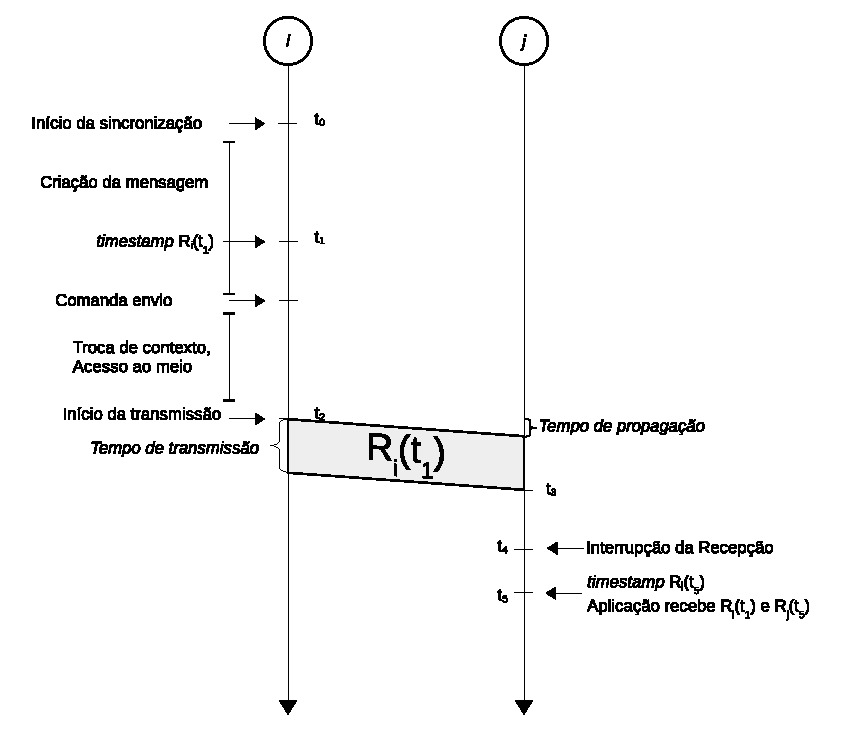
\includegraphics{./figuras/comparacao_mactime.eps}
 % comparacao_mactime.eps: 0x0 pixel, 300dpi, 0.00x0.00 cm, bb=
 \caption{Procedimento de leitura do \textit{timestamp} em n�vel de aplica��o}
 \label{fig:comp_apptimestamp}
\end{figure}




Visando corrigir esse problema, a leitura dos tempos pode ser efetuada em locais mais estrat�gicos. V�rios transmissores tem \textit{chips} capazes de modificar o conte�do da mensagem depois da transmiss�o ter sido iniciada, \textit{timestamps} na camada de acesso ao meio podem ser facilmente implementados nesses dispositivos para eliminar v�rios componentes de atraso.




\begin{figure}[h]
 \centering
 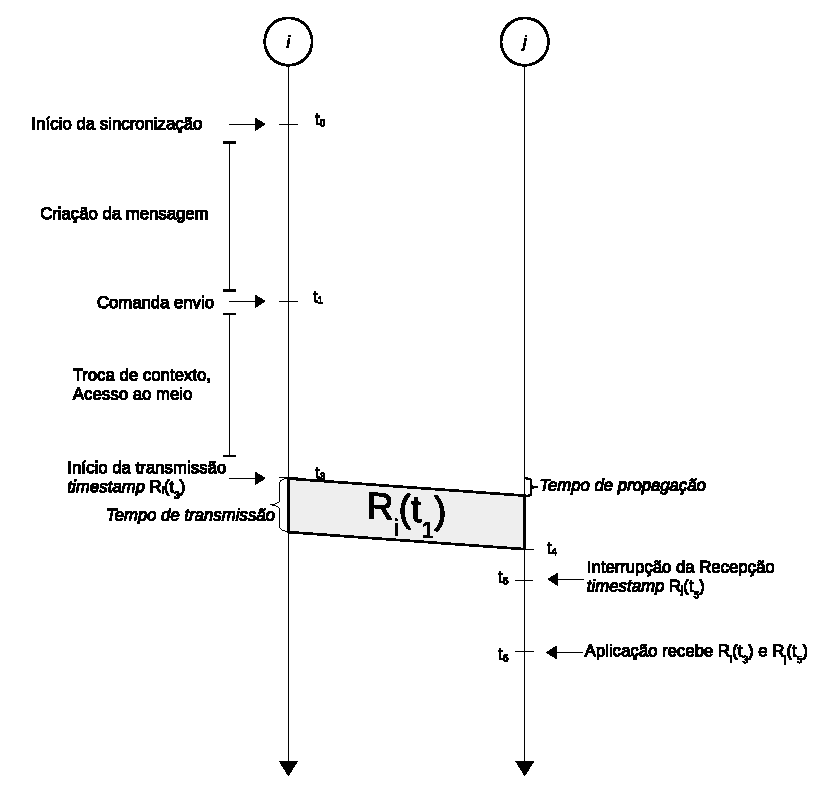
\includegraphics{./figuras/comparacao_mactime2.eps}
 % comparacao_mactime2.eps: 0x0 pixel, 300dpi, 0.00x0.00 cm, bb=
 \caption{Procedimento de leitura do \textit{timestamp} na camada MAC}
 \label{fig:comp_mactimestamp}
\end{figure}




Desta forma, quando � iniciado o processo de transmiss�o a mensagem vai para a fila de sa�da, por�m, quando os primeiros \textit{bits} s�o enviados o \textit{timestamp} � executado. Em um espa�o reservado no \textit{payload} do pacote � inserido uma informa��o adicional de quanto tempo a mensagem levou desde a cria��o at� o envio, procedimento este realizado pelo \textit{chip} de r�dio (uma interrup��o SFD - \textit{Start Frame Delimiter}). Isso permite que o receptor calcule e elimine os atrasos relacionados ao envio. Do lado do receptor � poss�vel usar MAC \textit{timestamp} no momento do recebimento e tamb�m eliminar os atrasos do receptor.

Na Figura \ref{fig:comp_mactimestamp} t�m-se a ilustra��o do procedimento de envio de mensagem de sincroniza��o utilizando \textit{timestamp} na camada MAC. O funcionamento do MAC \textit{timestamp} segue basicamente esse diagrama, onde o n� $i$ inicia o procedimento de envio mensagem de sincroniza��o em $t_0$, logo em seguida cria-se a mensagem e comanda-se o envio. No in�cio da transmiss�o � inserido na mensagem o tempo $t_3$, que � o mesmo instante do in�cio do envio dos dados. J� no lado do receptor, depois do atraso de propaga��o e do tempo de transmiss�o o �ltimo \textit{bit} chega, ent�o uma interrup��o � disparada no tempo $t_5$ junto com ela � registrada o \textit{timestamp} $t_5$.




O formato da mensagem do FTSP segue o modelo da Figura \ref{fig:pacote}. A mensagem come�a com um pre�mbulo, seguido do conjunto de \textit{bytes} de SYNC, um campo de dados e por fim um campo de identifica��o de erros CRC. O PREAMBLE � usado para sincronizar a frequ�ncia dos r�dios, o SYNC � utilizado para calcular o \textit{bit offset} e com isso alinhar os \textit{bytes} no receptor. Os \textit{timestamps} s�o armazenados no limite de cada \textit{byte} transmitido depois de SYNC, tando no envio quanto no recebimento. Os tempos s�o normalizados subtraindo um m�ltiplo inteiro correspondente ao tempo de transmiss�o. Somente o tempo final � inserido no campo de dados da mensagem.

\begin{figure}[H]
 \centering
 \includegraphics{./figuras/ftsp_packet.eps}
 % ftsp_packet.eps: 0x0 pixel, 300dpi, 0.00x0.00 cm, bb=0 0 221 17
 \caption{Formato da mensagem do FTSP}
 \label{fig:pacote}
\end{figure}






A forma como o \textit{timestamp} � realizado depende do modelo do \textit{chip} de r�dio. Pode ser dividido em dois tipos, orientado a \textit{byte} ou orientado pacotes. Nos \textit{chips} orientados a \textit{byte} como o CC1000 \cite{cc1000} (Mica2 e Mica2dot), geram interrup��o por cada \textit{byte} transmitido, essa interrup��o armazena no metadado da mensagem o \textit{timestamp} do momento em que o \textit{byte} foi transmitido ou recebido. Ao final da transmiss�o � poss�vel determinar um \textit{timestamp} �nico, calculando a taxa de transmiss�o e a m�dia dos \textit{timestamps}. Os \textit{chips} CC2420 \cite{chipcon20032} (MicaZ, TelosA, TelosB, TmoteSky) e RF230 (Iris) \cite{iris2006crossbow} s�o orientados a pacote, nesses r�dios ao inv�s de marcarem os tempos em cada \textit{byte} transmitido, fazem apenas uma marca��o para o pacote inteiro usando apenas uma �nica interrup��o SFD.









% Texto da tep 133:
% Several transceivers allow for modifying the contents of a packet after packet transmission is started. Packet-level time synchronization can be implemented very efficiently on such platforms.
% 
% Transmitter's story
% 
% When the communications stack services a TimeSyncAMSend.send command called with event timestamp t\_e, it stores t\_e (e.g. in a map with the pointer of the message\_t as key) and sets the designated timestamp field in the packet payload to 0x80000000.
% When the packet starts being transmitted over the communication medium, a corresponding hardware event is timestamped (e.g. an SFD interrupt). Let us denote this transmission timestamp with t\_tx. The difference of event timestamp t\_e and transmit timestamp t\_tx is written into the designated timestamp field in the payload of the packet (typically into the footer, since the first few bytes might have been transmitted by this time). That is, the information the packet contains at the instance when being sent over the communications medium is the age of the event (i.e. how much time ago the event had occurred).
% If an error occurs with timestamping the transmission or with writing the package payload after transmission has started, then the designated timestamp field in the packet payload will contain 0x80000000, indicating the error to the receiver.
% Receiver's story
% 
% The packet is timestamped with the receiver node's local clock at reception (e.g. with the timestamp of the SFD interrupt). Let us denote the time of reception with t\_rx. The reception timestamp is stored in the metadata structure of the message\_t [5].
% When the event time is queried via the TimeSyncPacket interface, the eventTime command returns the sum of the value stored in the designated timestamp field in packet payload and the reception timestamp, i.e. e\_t- e\_tx+e\_rx. This value corresponds to the time of the event in the receiver's local clock.
% The TimeSyncPacket.isValid command returns FALSE if the time value stored in the payload equals 0x80000000 or if the communications stack failed to timestamp the reception of the packet. Otherwise TRUE is returned, which indicates that the value returned by TimeSyncPacket.eventTime can be trusted.


\section{Escorregamento do Rel�gio}

\outline{
  Descrever os problemas relacionados ao clock drift.
  Como o FTSP corrige essa fonte de imprecis�o.
}

Como apresentado na Se��o \ref{subsec:conceitos}, os sensores de baixo custo apresentam rel�gios muito imprecisos. Cristais de diferentes n�s podem oscilar de forma ligeiramente diferente. Por exemplo, dado um \textit{mote} Mica que tem em sua especifica��o de f�brica a frequ�ncia de $7,3828~MHz$, por�m na verdade ele pode funcionar a $7,3827~MHz$ j� um outro \textit{mote} pode apresentar $7,3829~MHz$, isso gera 20 \textit{ticks} de erro por segundo, este erro acumulado pode atrapalhar a precis�o que se pretende oferecer em uma dada aplica��o. Esse comportamento causa a necessidade de ressincroniza��o em per�odos mais curtos. 

\begin{figure}[h]
 \centering
 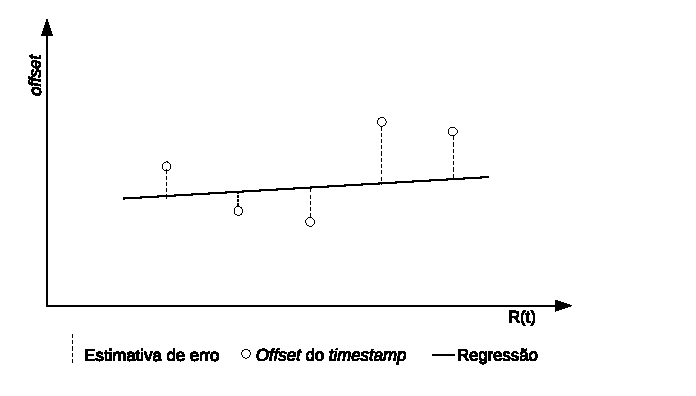
\includegraphics{./figuras/grafico_regressao.eps}
 % grafico_regressao.eps: 0x0 pixel, 300dpi, 0.00x0.00 cm, bb=
 \caption{Regress�o linear aplicada a \textit{timestamps}}
 \label{fig:regressao}
\end{figure} 

Regress�o linear � o m�todo mais utilizado para estimar o desvio do rel�gio de um n� para com o rel�gio da raiz \cite{maroti2004}. No processo de sincroniza��o um n� de refer�ncia ou \textit{root}, envia seu uma mensagem com seu pr�prio tempo, os receptores usam esse tempo para iniciar seu rel�gio local. Ent�o o \textit{root} passa a enviar periodicamente seu \textit{timestamp}, cada um dos receptores armazenam em uma tabela os tempos recebidos junto com o tempo de recebimento baseado no seu rel�gio local. A predi��o de erro � a diferen�a entre o tempo de refer�ncia do n� \textit{root} e a estimativa de tempo do n� receptor.

De acordo com \cite{capriglione2016}, usando regress�o linear � poss�vel predizer um padr�o pelo calculo dos pares de \textit{timestamps} recebidos, e utiliz�-los para compensar os erros. Uma linha de regress�o linear fornece a inclina��o necess�ria para estimar o tempo do n� \textit{root} no futuro, a Figura \ref{fig:regressao} ilustra esse processo. Assim, � poss�vel ajustar de forma mais suave a taxa de crescimento do rel�gio para algo mais pr�ximo na no��o global de tempo. No FTSP devido as limita��es de mem�ria dos dispositivos o tamanho padr�o das tabelas � 8 pares de \textit{timestamps}, os autores comprovaram em experimentos que a taxa de erro utilizando essa t�cnica � de $1.48\mu s$ em m�dia, quando desligado o recurso o erro passa a ser crescente e acumula com o tempo.






\section{Sincroniza��o Multi-saltos}

\outline{
\begin{itemize}
 \item Formato da mensagem de sincroniza��o.
 \item Gerenciamento de informa��o redundante.
 \item Elei��o do n� raiz.
 \item Evento: enviar/receber mensagem de sincronia. 
\end{itemize}

}



% \begin{figure}[h]
%  \begin{Verbatim}[numbersep=1pt,frame=single]
% typedef nx_struct TimeSyncMsg
% {
%  nx_uint16_t rootID;
%  nx_uint16_t nodeID; 
%  nx_uint8_t  seqNum;
%  nx_uint32_t globalTime;
%  nx_uint32_t localTime;
% } TimeSyncMsg;
% \end{Verbatim}
% \caption{Formato da mensagem de sincroniza��o}
% \end{figure}




%This section briefly describes the Flooding Time Synchronization Protocol (FTSP). For more detailed information, refer to \cite{maroti2004}.

% FTSP is a synchronization protocol for WSN that provides high accuracy, consumes few resources, uses little bandwidth and is fault-tolerant. It elects a node as root to provide the time reference for synchronization; if root failure is detected (using timeouts), another root is elected.
% Root and synchronized nodes send synchronization messages periodically, and receiving nodes use these messages to synchronize.
% Therefore, FTSP supports multi-hop networks.
% 
% Synchronization messages comprise a \textit{sender timestamp} which is the estimated global time and \textit{rootID} which is the network identifier of the root (where the node with the lowest ID is the chosen root).
% \textit{seqNum} is a sequence counter that is incremented each synchronization round; this field is used to verify the redundancy of messages \cite{maroti2004}.
% 
% All nodes think they are root when the network starts, so they broadcast synchronization messages to the network. 
% When they receive a synchronization message, they check who has the lowest ID: if the local ID is higher, this node gives up on being root and starts synchronizing.
% Another important check is the \textit{seqNum}.
% If it is greater than the local value \textit{highestSeqNum}, it means that this is a new synchronization message and starts the synchronization procedure.
% 
% The synchronization procedure consists of computing a linear regression \cite{elson2003} that will provide the clock skew (used to estimate the global time) in relation to the reference node.
% The last step is to forward its local (synchronized) time to other nodes. 


%%A mensagem de sincroniza��o compreende um \textit{timestamp} do emissor, que � estimativa de tempo global e \texttt{rootID} que � 


% \begin{figure}[h]
%  \centering
%  \includegraphics{./figuras/exemplo_ftps1.eps}
%  % exemplo_ftps1.eps: 0x0 pixel, 300dpi, 0.00x0.00 cm, bb=0 0 330 180
%  \caption{Exemplo do fluxo da rede com FTSP}
%  \label{fig:exemplo_ftsp1}
% \end{figure}


\begin{figure}[h]
\begin{Verbatim}[numbers=left,numbersep=1pt,frame=single]
event Radio.receive(TimeSyncMsg *msg){
  if( msg->rootID < myRootID )
      myRootID = msg->rootID;
  else if( msg->rootID > myRootID
    || msg->seqNum <= highestSeqNum )
      return;
  highestSeqNum = msg->seqNum;
  if( myRootID < myID )
      heartBeats = 0;
  if( numEntries >= NUMENTRIES_LIMIT
    && getError(msg) > TIME_ERROR_LIMIT )
      clearRegressionTable();
  else
      addEntryAndEstimateDrift(msg);
}
\end{Verbatim} 
 \caption{FTSP Receive Routine \cite{maroti2004} }%\vspace{0em}
 \label{figure1}
\end{figure}


A Figura \ref{figure1} mostra a rotina de recebimento de mensagens de sincroniza��o. 
As linhas 2 e 3 comparam o \texttt{rootID} da mensagem de sincroniza��o recebida com a informa��o local que o n� tem sobre que � o \textit{root} \texttt{myRootID}.
Se a mensagem recebida tem o \texttt{rootID} menor, o n� assume \texttt{rootID} como seu root.
As linhas de 4 a 7 ignoram as mensagens que tenham um \texttt{rootID} e \texttt{seqNum} menores, pois possuem informa��o irrelevante.
Se \texttt{seqNum} � maior, o valor de \texttt{highestSeqNum} � atualizado.
Linhas 8 e 9 fazem o n� \textit{root} desistir de ser a \textit{root} da rede quando existe um \texttt{rootID} menor que seu pr�prio ID.
No caso de \texttt{rootID} ser maior que o verificado se o \texttt{seqNum} � maior ou igual ao valor do \texttt{highestSeqNum}, esta checagem previne informa��es redundantes por que a mensagem ser� apenas usada quando o \texttt{rootID} for menor ou igual a \texttt{myRootID} e o numero maior que o valor de \texttt{highestSeqNum}.
Linhas 10 e 15 verificam se o tempo da mensagem est� em discord�ncia com a estimativa de tempo global mais recente, se � aplic�vel limpa a tabela de regress�o, se n�o, acumula a mensagem para calcular a regress�o linear e sincronizar.
As linhas 10 a 15 armazenam mensagens de sincroniza��o para calcular a regress�o linear e realizar a sincroniza��o.

% Figure \ref{figure1} shows the routine of receiving synchronization messages.
% Lines 2 and 3 compare the \textit{rootID} of the synchronization message with the local \textit{rootID}.
% If the message has a lower \textit{rootID}, the node assumes this \textit{rootID} as root.
% Lines 4 to 7 ignore messages with higher  \textit{rootID} and lower \textit{seqNum}.
% If \textit{seqNum} is higher, local \textit{highestSeqNum} is updated.
% Lines 8 and 9 makes a root node give up on being root when it has a \textit{rootID} lower than its own ID.
% In case the \textit{rootID} is larger it is checked whether the \textit{seqNum} is greater or equal to the value of \textit{highestSeqNum}, this check prevents information redundancy because the message will only be used when the \textit{rootID} is less than or equal to \textit{myRootID} and the number greater than the value of \textit{highestSeqNum}.
% Lines 10 to 15 verify if the time of a message is in disagreement with the earlier estimates of global time, if applicable clear the regression table, if not, accumulate synchronization messages to calculate the linear regression and synchronize.
%Lines 10 to 15 accumulate synchronization messages to calculate the linear regression and synchronize.



\begin{figure}[h]
   \begin{Verbatim}[numbers=left,numbersep=1pt,frame=single]
event Timer.fired() {
  ++heartBeats;
  if( myRootID != myID
    && heartBeats >= ROOT_TIMEOUT )
      myRootID = myID;
  if( numEntries >= NUMENTRIES_LIMIT
    || myRootID == myID ){
      msg.rootID = myRootID;
      msg.seqNum = highestSeqNum;
      Radio.send(msg);
  if( myRootID == myID )
      ++highestSeqNum;
  }
}
  \end{Verbatim}
  \caption{FTSP Send Routine \cite{maroti2004}}
  \label{figure2}
\end{figure}

A Figura \ref{figure2} mostra a rotina de envio de mensagem. 
Um n� decide tornar-se \textit{root} por que est� sem receber mensagens de sincroniza��o por \texttt{ROOT\_TIMEOUT} (linhas 3 a 5).
Um n� envia mensagens de sincroniza��o se ele � o \textit{root} ou se est� sincronizado (linhas 6 a 10).
Se um n� � o \textit{root}, ele tamb�m tem que incrementar seu \textit{highestSeqNum}.
% Figure \ref{figure2} shows the sending routine.
% A node decides to be root because has not received a synchronization message for ROOT\_TIMEOUT (lines 3 to 5).
% A node sends synchronization messages if it is root or has synchronized (lines 6 to 10).
% If a node is root, it also has to increment its \textit{highestSeqNum}. 


 
 
